\subsection{Общий подход к синтезу непрерывных систем на основе логарифмических частотных характеристик. Типовые желаемые логарифмические амплитудно-частотные характеристики}

Синтез системы
Направленный расчет, имеющий конечной целью отыскание: 1) рациональной структуры системы и 2) установление оптимальных величин параметров отдельных звеньев.
При множестве возможных решений, должен быть выбран критерий оптимизации – цена, точность, надежность, быстродействие, затраты энергии ...

При инженерном синтезе ставятся задачи:

Достижение требуемой точности.
Обеспечение приемлемого характера переходных процессов (задача демпфирования).
Решение первой задачи заключено в выборе средств повышающих точность системы (усилительных, изодромных блоков; каналов КУ; не 1ОС), т.е. фактически вида регулирования.
Решение второй задачи заключено в выборе оптимальных корректирующих средств.


\textbf{Метод логарифмических амплитудных характеристик}
Процесс синтеза включает в себя следующие операции:
\begin{enumerate}
    \item Построение располагаемой ЛАЧХ исходной системы $W_о$, состоящей из регулируемого объекта без регулятора и без корректирующего устройства.
    \item Построение НЧ части желаемой ЛАЧХ на основе предъявленных требований точности.
    \item Определение вида и параметров регулятора $K,K_i,\dots$:
    \begin{gather}
        W_{рег}(s ) = \cfrac{W_{\text{НЧ.ж}}(s)}{W_o(s)}  \\ L_{рег}(\omega)=L_{\text{НЧ.ж}}(\omega)-L_о(\omega).
    \end{gather}
    
    \item Уточнение ВЧ части желаемой ЛАЧХ на основе требований к запасу устойчивости~--- $L_{\text{НЧиВЧ.ж}}(\omega)$.
    \item Определение вида и параметров последовательного корректирующего устройства:
    \begin{gather}
        W_{\text{ПЗкор}} = \cfrac{W_{\text{НЧиВЧ.ж}}}{W_{per}W_о}\\
        L_{\text{ПЗкор}}=L_{\text{НЧиВЧ.ж}}-L_{рег}-L_о.
    \end{gather}
    \item Техническая реализация корректирующих устройств. В случае необходимости~--- перерасчет на эквивалентные параллельное звено или ОС.
    \item Поверочный расчет и построение переходного процесса.
\end{enumerate}


% Процесс синтеза обычно включает в себя следующие операции.
% \begin{enumerate}
%      \item Построение располагаемой ЛАХ. Под располагаемой ЛАХ понимается характеристика исходной системы управления, построенной исходя из требований, предъявляемых к точности режимов стабилизации или слежения, к мощности на выходе системы и т.п. Обычно под исходной системой понимается система, состоящая из управляемого объекта и управляющего устройства и не снабженная необходимыми корректирующими устройствами, обеспечивающими требуемое качество переходного процесса. Исходная система должна быть минимально-фазовой. Это значит, что передаточная функция разомкнутой исходной системы не должна иметь нулей и полюсов, расположенных в правой полуплоскости. Нулями называют корни полинома, стоящего в числителе передаточной функции, а полюсами~--- корни характеристического полинома.
    
%     \item Построение желаемой ЛАХ. Желаемой называют асимптотическую ЛАХ разомкнутой системы, имеющей желаемые (требуемые) статические и динамические свойства. Желаемая ЛАХ состоит из трех основных асимптот: низкочастотной, среднечастотной и высокочастотной. Кроме того, могут быть сопрягающие асимптоты, которые соединяют основные. При построении желаемой ЛАХ необходимо быть уверенным, что вид амплитудной характеристики полностью определяет характер переходных процессов и нет необходимости вводить в рассмотрение фазовую характеристику. Это будет выполняться в случае минимально-фазовых систем.
    
%     \item Определение вида и параметров корректирующего устройства. Наиболее действенным способом придания системе автоматического управления необходимых динамических свойств является введение в нее дополнительного элемента. Он исправляет, корректирует свойства исходной системы и называется корректирующим устройством. Корректирующее устройство включают в систему автоматического управления различным образом. Рассмотрим лишь один способ включения – последовательное включение корректирующего устройства в прямую цепь системы. В этом случае наиболее просто определяется передаточная функция корректирующего устройства, которую обозначим.
    
%     \item Техническая реализация корректирующих устройств. По виду ЛАХ необходимо подобрать схему и параметры корректирующего устройства последовательного типа.
    
%     Применение последовательных корректирующих устройств наиболее удобно в системах, у которых сигнал управления представляет собой напряжение постоянного тока. В этих случаях корректирующее устройство выполняют обычно из пассивных электрических четырехполюсников, обеспечивающих разнообразное преобразование сигнала. Еще больше возможности дают активные (т.е. с дополнительными источниками питания) электрические четырехполюсники постоянного тока.
    
%     \item Поверочный расчет и построение переходного процесса. Нельзя ожидать высокой точности результатов, полученных расчетным путем. Это объясняется прежде всего приближенностью используемого математического описания управляемого объекта и исполнительного элемента. Кроме того, содержат приближения и методы синтеза. Поэтому заключительным этапом расчета должен быть анализ синтезированной системы – определение показателей ее качества. А при физическом осуществлении системы нужна еще ее настройка.
    
%     Указанные обстоятельства не уменьшают значения теоретических расчетов. На основании расчетов выбирается структура корректирующего устройства и ориентировочные значения его параметров. Их отыскание экспериментальным путем значительно сложнее. Вместе с тем моделирование позволяет уточнить выбранные значения параметров.
% \end{enumerate}

\begin{figure}
    \centering
    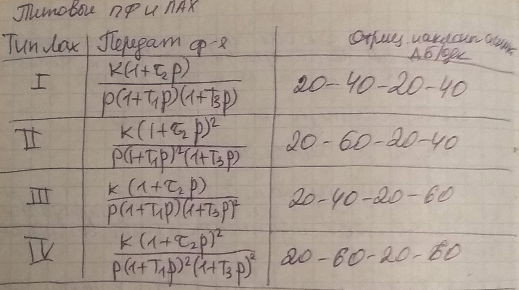
\includegraphics[width=0.7\textwidth]{images/pf.png}
\end{figure}